\graphicspath{{../04ClassicalPhysics/pics/}}

\chapter{Classical Physics}\label{ch:ClassicalPhysics}
\begin{quoting}
	I think we may ultimately reach the stage when
	it is possible to set up quantum theory without any reference to classical theory,
	just as we already have reached the stage where we can set up the Einstein
	gravitational theory without any reference to the Newtonian theory. But
	from the point of view of teaching students, I think one would always
	have to proceed by stages -- not expect too much from them, teach them
	first the elementary theories and gradually develop their minds; and
	that will always involve working from the classical theory
	first.
	
	P. A. M. Dirac, Lectures on Quantum Field Theory, Belfer Graduate
	School of Science, Yeshiva University, New York, 1966, p.43.
\end{quoting}

\lettrine[lines=2]{\color{darkocre}T}{he} concept of
\emph{operators}\index{Operator} extends the idea of functions. An unary numeric
function $f$ takes some numeric value $x$ as an input  and produces
another numeric value $y$:
\[
f\,x=y\quad \textrm{ or } \quad x\overset{f}{\longrightarrow} y\,.
\]
In mathematical jargon, $f$ \emph{maps} $x$ into $y$.

\begin{myprereq}{Prerequisite Knowledge}
	To fully understand the material of this chapter, readers should be comfortable with the following concepts:
	
	\begin{itemize}
		\item \phantom{phantom}
		\vspace{-0.5cm}
		\item State
		\item Dynamical equations
	\end{itemize}	
\end{myprereq}


\begin{figure}[htbp]
  \centering
  
\includegraphics[scale=1.0]{defaultFigureTemplate}
  \caption{Operators extend the idea of functions. (a) An unary
    function $f$ can be applied to a number $x$ to produce
    another number $y$. (b) An unary operator $\op{F}$ can be applied to a vector
    $\vec{a}$ to yield another vector $\vec{b}$.}
  \label{fig:arrowsOperatorGeneral}
\end{figure}

\section{System}\label{sec:System}
A part of nature that can be clearly isolated and studied is called a \emph{physical system}. An electron, an atom, a molecule, a crystal, a pendulum, a comet, a star – these are examples of physical systems of various degrees of complexity.

Often a physical system is a body or several bodies interacting with each other or with some external bodies. Figure \ref{fig:systemExamples} provides several examples of \emph{mechanical systems}. Let’s examine them in more detail.
\begin{figure}[htbp]
	\centering
	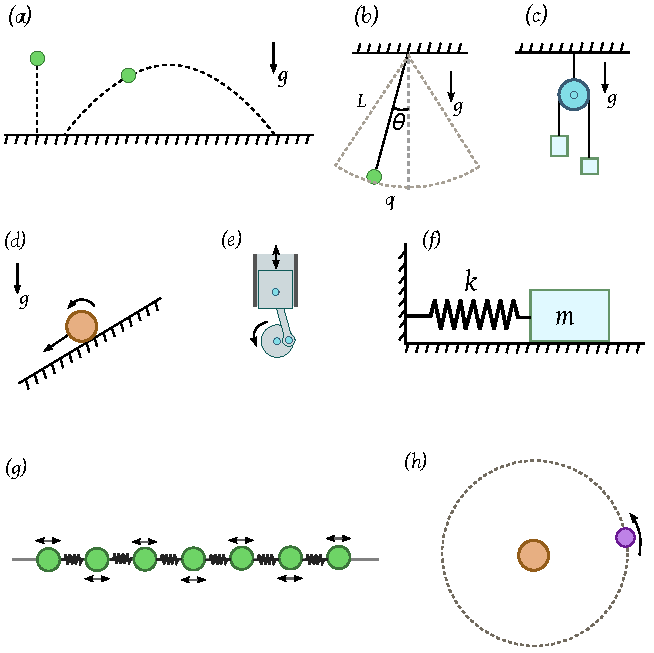
\includegraphics[scale=1.0]{systemExamples}
	\caption{Examples of mechanical systems. See text for explanation..}
	\label{fig:systemExamples}
\end{figure}
\renewcommand{\labelenumi}{(\alph{enumi})}
\begin{enumerate}
	\item \emph{Free falling body}: An elastic body falls down vertically under the
	force of gravity, bounces back, goes up and then down to repeat the
	bounce again and again. Also, a projectile launched at an angle.
	\item \emph{String pendulum}: A compact body is attached to a string
	of fixed length. It is allowed to swing back and forth without
	experiencing air friction.
	\item \emph{Atwood machine}: Two bodies with slightly unequal masses
	are connected with a non-stretchable string going over a
	frictionless pulley.
	\item \emph{Inclined plane}: A solid cylinder rolling down an
	inclinded plane.
	\item \emph{Piston}: A system of three bodies (cylindrical
	crankshaft, rod, and piston) connected in a way that locks rotation
	of a cylinder and the vertical motion of the piston.
	\item \emph{Spring oscillator}: A body, attached to a spring, is
	allowed to slide left and right across a frictionless surface.
	\item \emph{Linear chain of oscillators}: A set of pairwise
	interconnected identical bodies; the allowed motion happens along
	the horizontal axis.
	\item \emph{Sun and planet}: A planet circling around the sun.
	
\end{enumerate}
We will study oscillator and circular motion in great detail.

\subsection{Configuration}
In mechanics, \emph{configuration} means a formal way to describe the
arrangement of a system at a given time.

The behavior of a system in time can be described by specifying its
\emph{configuration} as the function of time. In relatively simple
systems, configuration may consist of a set of coordinates that uniquely
determine the arrangement of bodies in the system. For example, the
configuration of a pendulum can be given by a single coordinate --- the
length of the arc $q$. Of course, as the pendulum swings, both
Cartesian coordinates $x$ and $y$ are changing, but not independently,
due to the relation
\begin{equation*}
	x^2 + y^2 = L^2\, .
\end{equation*}
Given $x$, we can find $y > 0$ as $y = +\sqrt{L^2 - x^2}$, thus
reducing the number of required coordinates.

Consider another example, shown in the Figure
(\ref{fig:coupledSystem})(a): a system of
two bodies, connected with each other using ideal springs with
stiffness $k$, and each body is connected to a rigid wall.
\begin{figure}[htbp]
	\centering
	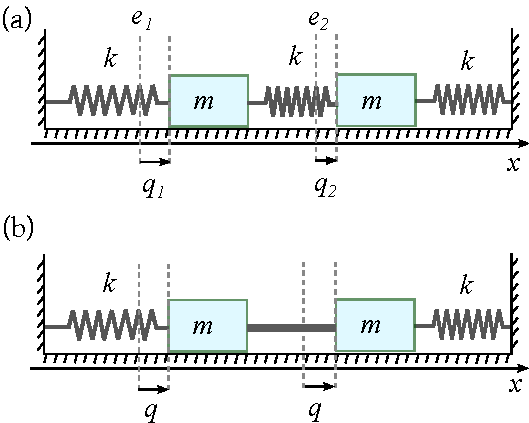
\includegraphics[scale=1.0]{coupledSystem}
	\caption{(a); (b).}
	\label{fig:coupledSystem}
\end{figure}

When the system is in equilibrium, the bodies occupy positions on the
horizotal axis denoted as $e_1$ and $e_2$. During motion, the position
of the first body changes by
\begin{equation*}
	q_1(t) = x_1(t) - e_1\, ,
\end{equation*}
and similarly for the second body: $q_2 = x_2 - e_2$. It is important
to realize, that although the two bodies are connected with a spring,
they can still move with different velocities, and have different
displacements $q_1 \ne q_2$. Indeed, we can set the system in motion
by moving each body independently and then releasing them. Contrast
this with the situation, shown in the Figure
(\ref{fig:coupledSystem})(b), where the bodies are connected with a
rigid rod, fusing two masses into essentially a single body. In this
case only a single displacement $q$ is required to specify the
configuration of the system.

\subsection{Qoordinates}
The coordinates specifying the configuration of a system do not
have to be Cartesian. In the example of a pendulum, the configuration
can be conveniently given by the length of the arc $q=L\theta$, see
Figure (\ref{fig:systemExamples})(b).

Consider another example, shown in the Figure
(\ref{fig:systemExamples})(h): Two bodies interact
gravitationally. In this problem, it turns out, the equations
describing the motion of the system are simpler if, instead of the
usual positions $x_1$ and $x_2$ we use the relative distance
\begin{equation*}
	q_1 = x_2 - x_1
\end{equation*}
and the position of the center of mass
\begin{equation*}
	q_2 = (m_1x_1 + m_2x_2)/(m_1 + m_2),
\end{equation*}
where $m_1$ and $m_2$ are the masses of the bodies.

We thus come to the idea of \emph{generalized coordinates} --
arbitrary coordinates completely specifying the configuration of a
system. Generalized coordinates can be based on positions, angles, or
some combinations of those.

\subsection{Degrees of Freedom}
\emph{Degree of freedom} is a separate independent motion of a
mechanical system. Each independent motion corresponds to the change
in time
of a separate generalized coordinate. The number of degrees of freedom
is the number of
generalized coordinates required to completely specify the
configuration of a mechanical system at different moments of time.

Take, for example, a pendulum, shown in the Figure
(\ref{fig:degreeOfFreedomPendulum}). In general Cartesian coordinates,
all three coordinates $x$, $y$, and $z$ will be changing in
time. However, only a single generalized coordinate $q(t)$ --- the
length of the arc -- is required to fully describe the configuration,
and thus the motion, of this mechanical system. The number of degrees
of freedom, in this example, equals 1.

\begin{figure}[htbp]
	\centering
	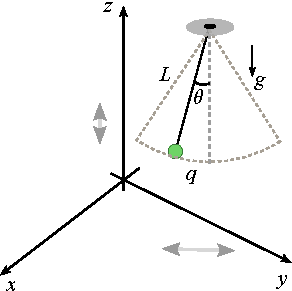
\includegraphics[scale=1.0]{degreeOfFreedomPendulum}
	\caption{A pendulum has one degree of freedom, despite the fact
		that all three Cartesian coordinates can be changing during its motion.}
	\label{fig:degreeOfFreedomPendulum}
\end{figure}




\section{Oscillator}\label{sec:Oscillator}
The model of an oscillator is extremely important. It appears in
various guises in almost all physical theories. Let's study it in details.

\begin{figure}[htbp]
	\centering
	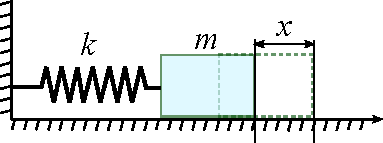
\includegraphics[scale=0.9]{Oscillator}
	\caption{A mechanical model of an oscillator: A body attached to an
		ideal spring.}
	\label{fig:Oscillator}
\end{figure}


Consider a body with the mass $m$ is attached to a spring with the stiffness
$k$. The body is allowed to move across a frictionless
surface.  The force required to strech a spring by the amount $x$
is given by the Hooke's law
\[
F=kx.
\]
This is the force applied \emph{to the spring}. The force created
\emph{by the spring, and applied to the attached body}, is of equal
magnitude but points in the opposite direction.

When the body is displaced from its equilibrium position,
by stretching or compressing the spring, and then released, it will
undergo periodic motion. During this motion, the position, velocity,
kinetic energy of the mody, and the potential energy of the spring
will be constantly changing.

To remind, the kinetic energy of a body is

\[
E_{k}=\frac{mv^{2}}{2}, \textrm{ or } K = \frac{p^2}{2m}\,.
\]
The potential energy of a spring, stretched or compressed by the
amount $x$ is given by

\[
E_{p}=\frac{kx^{2}}{2}, \textrm{ or } \Pi = \frac{kq^2}{2}\,.
\]


\section{State}\label{sec:State}
\emph{State} of a system is the \emph{minimal} collection of observables which is, in
certain sense, \emph{complete} and \emph{self-sufficient}. State is 
"all there is to know" about a system. If the state of a system is known at one
moment of time $t_0$, then we should be able to determine the state
at any later moment of time $t$. In classical mechanics the pair of
observables $(x, p)$ defines the state of a mechanical system.

\emph{State} is the minimal set of quantities describing mechanical
system and sufficient to predict
their future values from their initial values. State is an important
concept not only mechanics, but in other areas of physics.
Let's elaborate, using the oscillator as an example.

Suppose that at the moment of time $t_{0}$ the position of an oscillator
is $x_{0}$ and its velocity is $v_{0}$. To find their values at
some later time $t>t_{0}$, we can go iteratively in small steps, calculating
how much the position and the velocity change after each successive
tiny interval of time $\delta t$. The first iteration results in
the updated value of position
\[
	x_{1}=x_{0}+v_{0}\delta t.
\]
The second, and every other, iteration looks very similar:
\[
	x_{2}=x_{1}+v\delta t\,.
\]
Now it is important to realize that we can no longer use the same initial
velocity $v_{0}$ in the second iteration, because the velocity itself
changes. Thus, we must update the value of the velocity as well. This
is done by using acceleration:
\[
	v_{1}=v_{0}+a_{0}\,.
\]
After that, we can find the second iteration of the position:
$x_{2}=x_{1}+v_{1}\delta t$. To keep this scheme going, we must be
able to update the value of the acceleration, because it is also changing.
It appears then, we need some quantity that allows to find the next
step:
\[
	a_{1}=a_{0}+b_{0}\delta t\,.
\]
Fortunately, \emph{this is not needed!} At this point we can use the laws of motion.
For example, Newton's second law gives the acceleration in terms of the known force acting on the object:
\begin{equation}
	a=\frac{F}{m}.
\end{equation}
\begin{important}
	Forces don't depend on acceleration.
\end{important}

All known forces in physics depend on positions or distances and--
sometimes-- velocities of bodies. For example, the force of the spring $F=-kx$
depends only on the coordinate $x$. The force of gravitational interaction $F=GMm/r^2$
and the Coulomb force between two charges $F=kQq/r^2$ depend on the distance
$r$ between the bodies. The force acting on an electron moving through
a magnetic field--known as Lorentz force\index{Lorentz!force}-- equals $F=qvB$ and 
depends on the electron's velocity (and the field's strength $B$). 
No known forces depend on acceleration. This fact leads to an important conclusion:
It is enough to know position and velocity of an object at time $t_{0}$,
in order to find their values at any later moment of time $t>t_{0}$.
Obviously, position and velocity at any previous moment of time can
be found in the similar way.

Thus, we do not need to advance the acceleration by calculating its
small change $\delta a=b\delta t$, we can simply calculate it from
the law of motion:
\begin{equation}
	a_{n}=\frac{F(x_{n},v_{n})}{m}\,.
\end{equation}

This formula says that the acceleration at the iteration step number
$n$ is found from the values of the position $x_{n}$ and the velocity
$v_{n}$ at the same step. Given the velocity, we can advance the
postion, and given the acceleration, we can advance the velocity.
Then we recalculate the new value for the acceleration and repeat,
until we reach the final time $t$.

The preceding discussion demonstrates that in Newtonian mechanics
\emph{the state of a mechanical system} is given by a pair of quantities
-- $(x,v)$. There are alternatives to the Newtonian mechanics, and,
correspondingly, there are alternatives to the mechanical state. The
first such alternative is Hamiltonian dynamics.

\subsection{State Evolution: Newtonian Approach}
We will now apply the ideas and formulas of Newtonian mechanics to an
oscillator. We will calculate the motion of the oscillator in time
using a simple method of \emph{state evolution}. Specifically, we will
setup two simple equations -- one for position and one for velocity.

The equation for position is trivial and amounts to the definition:
\[
\frac{\delta x}{\delta t} = v\,.
\]
The equation for velocity follows from the second law of Newtonian
dynamics:
\[
\frac{\delta v}{\delta t} = \frac{F}{m} = -\frac{kx}{m}\,.
\]
Here we used the expression for the spring force $F=-kx$ acting
\emph{on the body} from the side of the spring.

Suppose we know the \emph{initial state} of the oscillator
$(x_0, v_0)$ at time $t_0=0$. When the clock makes a single tick after
a tiny time interval $\delta t$ the body will move to a new position
\[
x_1 = x_0 + v_0\delta t
\]
and the velocity will change due to the action of the spring:
\[
v_1 = v_0 -\frac{kx_0}{m}\,.
\]
Thus, after a single tick of the clock the state of the oscillator
will evolve from $\ket{\xi}_0=(x_0, v_0)$ to $\ket{\xi}_1=(x_1, v_1)$. At this point we can
keep repeating the steps to calculate the state after any number of
ticks, up to the desired time $t=N\delta t$.

We can now formalize the recipe for evolution of the state, writing it as a mathematical relation:
\[
\ket{\xi}_{new} = f\,\ket{\xi}_{old}\,,
\]
where 
\[
\ket{\xi}_{new}=(x_{new}, v_{new}) = (x_{old}+v_{old}\delta t, v_{old} - kx_{old}/m)\,.
\]
\begin{figure}[htbp]
	\centering
	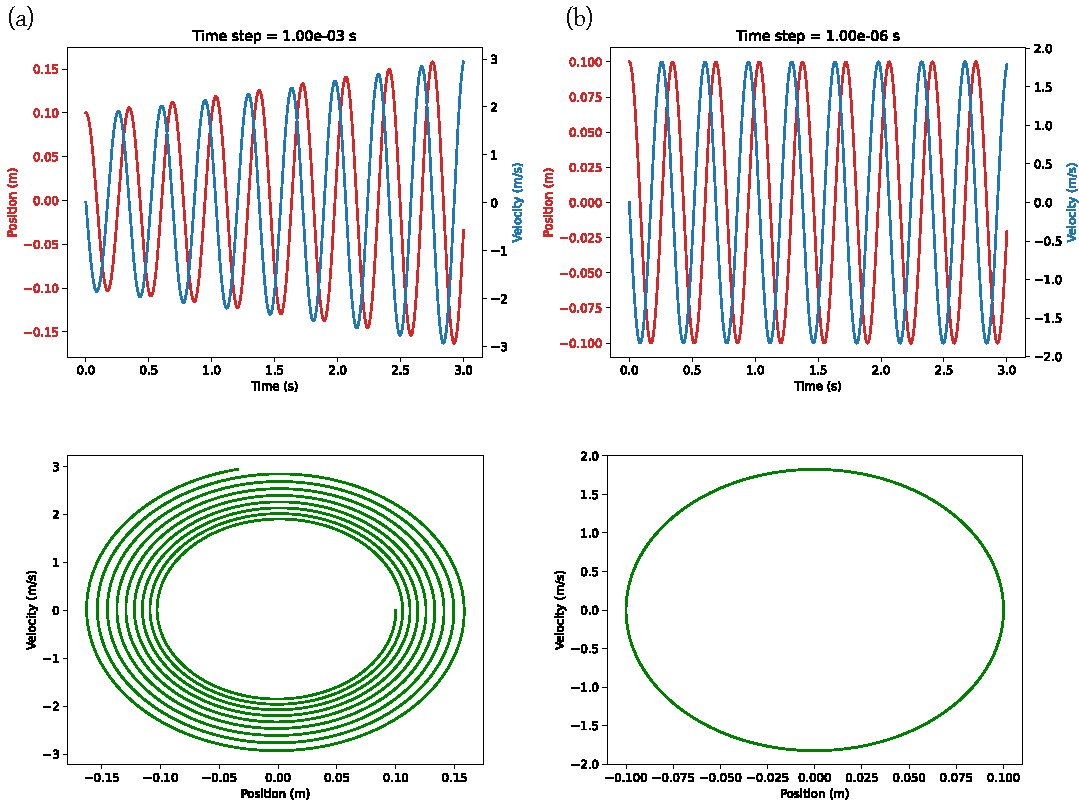
\includegraphics[scale=0.65]{newtonianStateEvolution}
	\caption{First row: Position (red curve, left axis) and velocity (blue
		curve, right axis) as functions of time. Second row: Velocity vs position.
		(a) Calculations with time step of 1 millisecond. (b) Calculations
		with time step of 1 microsecond.}
	\label{fig:newtonianStateEvolution}
\end{figure}

Using this simple approach, we can calculate the state $\ket{\xi}=(x, v)$ of the
oscillator for any moment in the future or past. Figure
\ref{fig:newtonianStateEvolution} shows two example results. The first
result, in the column (a), demonstrates that we must be careful with
the step size $\delta t$ of the time. If it is not sufficiently small,
the inherent error of the method accumulates quickly, resulting in
wrong behavior, such as the gradual increase of velocity and
oscillation amplitude. The column (b) of Figure
\ref{fig:newtonianStateEvolution} demonstrates the expected behavior
of the oscillator -- periodic change of position and velocity with constant amplitudes.

\section{Dynamics}\label{sec:Dynamics}
\emph{Dynamics} is the study of state evolution of various systems subject to known interactions. 
Physical systems of interest can be mechanical, like the ones given in example above (WHERE? REF), or  "non-mechanical" like electromagnetic field or even gravitational field. One can also explore dynamics of quantum systems.
 
The central equation in dynamics describes the state change in time due to known \emph{laws of dynamics}:
\[
\partial_t\,\ket{\xi}=\op{D}_{int}\,\ket{\xi}\,.
\]
We will explore three main variants of classical dynamics: Newtonian, Hamiltonian, and Lagrangian. They will prepare us for better understanding \emph{quantum dynamics}.

Newtonian dynamics is based on the notion of \emph{force} as the driver of interaction:
\[
(\partial_t\,x,\,\partial_t\, v)=(v, F/m)\,.
\]
Both Hamiltonian and Lagrangian mechanics rely on the notion of energy. 

\section{Hamiltonian}\label{sec:Hamiltonian}
\emph{Hamiltonian} is the expression for total energy of a system in terms of position and momentum. For example, using the non-relativistic expression for momentum $p=mv$, the Hamiltonian of  an oscillator can be written as
\begin{equation}
	H = \frac{p^2}{2m} + \frac{kx^2}{2}\,.
	\label{eq:OscillatorHamiltonian}
\end{equation}

Hamiltonian, denoted simply as $H$, still means the total energy. The only difference between $H$ and $E$  is the emphasis on the use of momentum in $H$ instead of velocity.

\begin{important}
	Momentum is more fundamental than velocity.
\end{important}

Although velocity feels more intuitive and closer related to our visual perception of motion, momentum is a more \emph{fundamental quantity} in physics. There is a \emph{conservation of energy and momentum} law, but there is no law of the conservation of velocity.

\subsection{Phase Space}
Hamiltonian dynamics uses position $x$  and momentum $p$  to study motion. For an isolated system with conserved energy (constant Hamiltonian), the expression for the Hamiltonian establishes the relationship between $x$ and $p$  for all moments of time. For example, using the Hamiltonian for an oscillator (\ref{eq:OscillatorHamiltonian}), we can rewrite it as follows:
\begin{equation}
	1=\frac{p^2}{(2mH)}+\frac{x^2}{(2H/k)}\,.
	\label{eq:phaseSpaceEllipse}
\end{equation}
This has the same form as the equation of an ellipse in Cartesian axes $(x,y)$:
\[
1=\frac{y^2}{b^2}+\frac{x^2}{a^2}\,.
\]
The area of such an ellipse with the semi-axes $a$ and $b$ is $A=\pi ab$. For $a=b$ an ellipse becomes a circle with the area $A=\pi R^2$.

The equation (\ref{eq:phaseSpaceEllipse}) describes an ellipse in a special $xp$-plane, every point of which can be specified by a pair of values $(x,p)$. Such a plane is called \emph{phase space}. It plays an important role in Hamiltonian dynamics.

The maximum value of the momentum is $p_{max}=\sqrt{2mH}$ and the maximum value for the displacement of the body is $x_{max}=\sqrt{2H/k}$. It turns out, the \emph{area of the ellipse in the phase space is directly proportional to the total energy of the oscillator}:
\[
A=\pi x_{max}p_{max}=2\pi H\sqrt{m/k}\,,
\] 
or
\[
H=\frac{A}{2\pi}\sqrt{\frac{k}{m}}\,.
\]
This important relationship will be used later when we will study quantum properties of the oscillator.

\subsection{Hamiltonian Equations}
Hamiltonian dynamics tracks the time dependence of position $x_t$ and momentum $p_t$. The pair of values $(x,p)$ represents the \emph{state in Hamiltonian dynamics}. Indeed, since there is a unique relationship between the momentum and velocity (e.g. $p=mv$ for non-relativistic speeds $v\ll c$, $c$ — speed of light), the knowledge of $\ket{\xi}=(x,p)$ is equivalent to  the knowledge of $\ket{\xi}=(x,v)$ which is the state in Newtonian dynamics. Put differently, the pair $(x,p)$ provides the same complete description of the system as $(x, v)$.

The main difference between Newtonian and Hamiltonian approaches, is that in the latter the equations for the rate of change of $x$ and $p$ are \emph{explicitly tied to the Hamiltonian}— to the form of the energy expressed in terms of position and momentum. In other words, the equations for $\partial_t\,x$ and $\partial_t\,p$ are written in the following  form:
\[
\partial_t\, x = \op{X}\,H\,\quad\textrm{ and }\quad \partial_t\, p = \op{P}\,H\,.
\]
where $\op{X}$ and $\op{P}$ are some \emph{rules} for calculating velocity $v=\partial_t\, x$  and force $F=\partial_t\,p$ from Hamiltonian $H$. Mathematically, $\op{X}$ and $\op{P}$ must be \emph{operators}: they take the function $H(x,p)$ and calculate the functions $v(x,p)$ and $F(x,p)$.

Let’s use the oscillator model to see how exactly these equations look like. 

\begin{exercise}
	Show that for an oscillator $v=p/m=\partial_p\, H$ and $F=-kx=-\partial_x\, H$.
\end{exercise}
Using the results of the exercise, we can conclude that for the oscillator the equations of Hamiltonian dynamics are
\begin{align}
	\label{eq:HamiltonianEquationsA}
	\partial_t\,x & =  \partial_p\, H\,,\\
	\partial_t\,p & = -\partial_x\, H\,. 
	\label{eq:HamiltonianEquationsB}
\end{align}
The equations (\ref{eq:HamiltonianEquationsA}) and (\ref{eq:HamiltonianEquationsB}) are called \emph{Hamiltonian equations of motion}.

\begin{exercise}
	In special theory of relativity it is shown that the energy $E$ and momentum $p$ of any particle are related to its mass $m$ as follows:
	\[
	m^2=E^2-p^2\,.
	\]
	(Special units must be used for this equation to hold. In these special units all velocities are measured as the fractions of the speed of light, while energy, momentum, and mass are all measured in the same units.)
	
	Starting from the Hamiltonian of a relativistic particle 
	\[
	H^2=p^2+m^2\,,
	\]
	show that the momentum depends on velocity as
	\[
	p=\frac{mv}{\sqrt{1-v^2}}\,.
	\]
	Then show that momentum and energy are related as $p=Ev$.
\end{exercise}

\subsection{Solving Oscillator Equations}
We will now find the exact time dependence of both position $x_t$ and momentum $p_t$ of the oscillator. To do that, we will need to take another look at the evolution of the state of the oscillator in phase space.

The state of an oscillator corresponds to a point in the phase space. This point can be mathematically represented either as a vector $\ket{\xi}$ connecting the origin and the point, or as a pair of values $(x,p)$ . Two descriptions are equally valid. Moreover, the pair of values $(x,p)$  can be considered as the components of the vector $\ket{\xi}$. 

As the time progresses, the position and momentum of the oscillator change, but the tip of the arrow $\ket{\xi}$ remains on the ellipse, corresponding to a constant energy $H$. The axes of "ordinary" phase space have different physical units, whereas the "usual" Cartesian axes $(x,y)$ have the same units and are equivalent in their meaning. It is convenient to temporarily introduce \emph{normalized} energy, position, and momentum.

First, let us express the energy of the oscillator in terms of the rest-energy of the electron $E_e=m_e c^2$. Then the Hamiltonian of the oscillator (its total energy) can be written as $H=\bar{H}E_e$. If the rest-energy and Hamiltonian are measured in Joules, then $\bar{H}$ is a number without units. (COOKIES?)

Next, we will introduce a "scale" for position of the oscillator. Specifically, we will denote $x_e=\sqrt{2E_e/k}$ as the amplitude of the oscillation when the total energy is equal to $E_e$. This amplitude is measured in meters. Then the displacement can be written as $x=\bar{x}x_e$, where $\bar{x}$ is a number without units.

Finally,  we will introduce a "scale" for momentum of the oscillator: $p_e=\sqrt{2mE_e}$ as the amplitude of the oscillation when the total energy is equal to $E_e$ . (\emph{Note}: the mass $m$  in $\sqrt{2mE_e}$ is the mass of the body attached to the spring, \emph{not} the mass of the electron) The "scale" $p_e$  is measured in kilograms times meters per second -- the usual units for momentum. Therefore, the momentum of the oscillator can be written as $p=\bar{p}p_e$, where $\bar{p}$ is a number without units. 

Substituting $H=\bar{H}E_e$ , $p=\bar{p}p_e$, and $x=\bar{x}x_e$  into the expression for the Hamiltonian, we obtain
\[
\bar{H}E_e=\frac{p_e^2}{2m}\bar{p}^2+\frac{kx_e^2}{2}\bar{x}^2=E_e\bar{p}^2+E_e\bar{x}^2\,,
\]
from which follows a very simple relationship between pure numbers: $\bar{H}=\bar{p}^2+\bar{x}^2$. This equation describes a circle in \emph{normalized phase space} $(\bar{x}, \bar{p})$ . The tip of the \emph{normalized state} vector $\ket{\bar{\xi}}=(\bar{x}, \bar{p})$ performs clock-wise circular motion. If we denote the magnitude of the angular speed of this motion as $\omega$, then we can use the familiar equation for the circular motion:
\[
\partial_t\,\ket{\bar{\xi}} = -\omega\op{J}\ket{\bar{\xi}}\,.
\]
The minus sign in the right-hand side is due to the clock-wise rotation of the state vector $\ket{\bar{\xi}}$.

The left side of the last equation is a two-component vector $(\partial_t\,\bar{x}, \partial_t\,\bar{p})$. The right hand side is also a vector with components $-\omega\op{J}\ket{\bar{\xi}}=(\omega\bar{p}, -\omega\bar{x})$. The equality of vectors means the equality of their components: 
\[
\partial_t\,\bar{x}=\omega\bar{p}\quad\textrm{ and }\quad\partial_t\,\bar{p}=-\omega\bar{x}\,.
\]
Let’s examine the equality $\partial_t\,\bar{x}=\omega\bar{p}$. The left hand side can be expanded as follows: 
\[
\partial_t \bar{x}=\frac{\delta \bar{x}}{\delta t}=\frac{\delta (x/x_e)}{\delta t}=\frac{1}{x_e}\frac{\delta x}{\delta t}=\frac{v}{x_e}\,.
\]
The right hand side can be written as $\omega \bar{p}=\omega\frac{p}{p_e}=\frac{\omega m v}{p_e}$. We showed that 
\[
\frac{v}{x_e}=\frac{\omega m v}{p_e}
\]
and consequently, $\omega = p_e/(mx_e)$. The conclusion is very important: \emph{The angular speed of rotation of normalized state arrow  for harmonic oscillator is constant}. The oscillator returns into its initial state with the period $T=2\pi/\omega$.

When we plug in the expression for $x_e$ and $p_e$ in terms of the energy $E_e$ and the parameters of the oscillator $k$ and $m$, we will arrive at the following equations for the frequency and period of oscillatory motion:
\[
\omega=\sqrt{\frac{k}{m}}\quad\textrm{ and }\quad T=2\pi\sqrt{\frac{m}{k}}\,.
\]
Now we can write the components of the normalized state vector as
\[
\bar{x}=\sqrt{\bar{H}}\cos\,(\omega t)\quad\textrm{ and }\quad \bar{p}=-\sqrt{\bar{H}}\sin\,(\omega t)\,.
\]
The minus sign for momentum comes from the fact that the "circular motion" in normalized phase space is clockwise and $\omega < 0$.

Going back to "normal" energy, position, and momentum is easy. Indeed, we first find $x_t =x_e \sqrt{H/H_e}\cos\,(\omega t)$ which simplifies to simple harmonic motion:
\[
x_t =\sqrt{2H/k}\cos\,(\omega t)\,.
\] 
Similarly for momentum: $p_t=-\sqrt{2mH}\sin\,(\omega t)$.

\begin{exercise}
	Show that for harmonic oscillator
	\[
	\Delta x = \sqrt{\langle x^2\rangle-(\langle x\rangle)^2} = \sqrt{H/k}\,,
	\]
	and
	\[
	\Delta p = \sqrt{\langle p^2\rangle-(\langle p\rangle)^2} = \sqrt{mH}\,.
	\]
	Then show that $\Delta x\Delta p=H/\omega$.
\end{exercise}

\section{Lagrangian}\label{sec:Lagrangian}
\emph{Lagrangian} of a physical system is a special function of its coordinates and velocity that captures some aspect of energy, not covered by the total energy or Hamiltonian. For many systems Lagrangian describes the \emph{imbalance} of kinetic energy over the potential energy. For example, the Lagrangian of the oscillator is
\begin{equation}
	L = E_k - E_p = \frac{mv^2}{2}-\frac{kx^2}{2}\,.
	\label{eq:oscillatorLagrangian}
\end{equation}
\begin{important}
	Unlike total energy, Lagrangian is generally not conserved.
\end{important}
\begin{exercise}
	Using the results for $x_t$ and $p_t$ from Hamiltonian dynamics for the oscillator, find the explicit form of its Lagrangian as the function of time.
\end{exercise}
The units for Lagrangian are the same as the units for energy or
Hamiltonian (Joules in International System SI), but the meaning and the role
of Lagrangian is what sets it apart from other functions of the state of a mechanical system.
Lagrangian is used to find the \emph{equations of motion} for the system. For each independent coordinate (e.g. $x$, $y$, or $z$) one finds a separate equation of motion using Lagrangian. Let’s see how this works for the oscillator.

The first step is to extract momentum $p=mv$ from the Lagrangian. Looking at the expression (\ref{eq:oscillatorLagrangian}), we find $p=\partial_v\,L$. Next, we should find the "force" acting on the body. The force will allow us write down Newton’s second law in the form $F=\partial_t\,p$. Again, from the expression (\ref{eq:oscillatorLagrangian}), we find $F=-kx=\partial_x\,L$.

Finally, rewriting $F=\partial_t\,p$  in terms of the Lagrangian, we arrive at Euler-Lagrange equation:
\[
\partial_t\,\left(\partial_v\,L\right)=\partial_x\,L\,.
\]
The dynamical equations for a general system will have the same form.

\begin{mybio}{Lagrangian in Qoordinates}
	The power of Lagrange approach to mechanics lies in its indifference to the type of coordinates used to describe mechanical system. It is often convenient to use some \emph{generalized coordinate} $q$ instead of Cartesian coordinate $x$ (or $y$ and $z$). \emph{Generalized velocity} is then $\nu=\partial_t\,q$. In terms of generalized variables, Euler-Lagrange equations still have the same form:
	\[
	\partial_t\,\pi = \partial_q\,L
	\]
	where $\pi=\partial_\nu\, L$ is \emph{generalized momentum}.
\end{mybio}

\subsection{Stationary Action Principle}
Euler-Lagrange equations — the equations of motion for a system with specified Lagrangian $L(x,v)$ — are more rigorously derived using an important physical principle known as the \emph{Stationary Action Principle}. Sometimes it is called \emph{"principle of least action"} and has a special case known as \emph{"principle of least time"}. However, the proper name is the stationary action principle.
To understand the idea behind the stationary action principle we must recall the concept of a functional, and in particular the \emph{action functional} .

Although mathematically Lagrange function $L(x,v)$ depends on two inputs --
position and velocity -- it is usually transformed into a function of
time only $L_t$ and then used to calculate an imporant physical
quantity called \emph{action}. We will study a specific example of
this below.

Simply speaking, action is the \emph{imbalance of energies accumulated
	during the particular motion of a system}. In practice it works as
follows: One chooses a particular way a mechanical system moves by
choosing a particular dependence of position on time $x_t$. This
function immediately determines the velocity $v(t) = \partial_t
x$. Then we can calculate kinetic and potential energies and
corresponding Lagrange function as a function of time
\[
L_t = E_k(t) - E_p(t)\,.
\]
With this function, we can calculate action -- the total accumulated
imbalance of energies -- during a specific period of time:
\[
A = \int \delta t L_t\,.
\]
\begin{mybio}{Stationary Time Principle}
	When a system has constant Lagrange function, then
	the total action becomes proportional to total time. In this case
	the principle of least action is known as the \emph{principle of
		extreme (least or maximal) time}.
\end{mybio}
One can try \emph{any type of physically allowable motion} $x_t$  and
calculate the total action $A$. Different ways of motion will result in different
values for the total action. Turns out, there is one unique function
$x^*_t$ for which the value of action $A$ is \emph{stationary} or
\emph{extreme} -- either maximal or minimal and \emph{insensitive to small
deviations} of the motion $x_t$ from its "true" form $x^*_t$. This
is the essense of the \emph{stationary action principle}. It is better
to demonstrate it using an example.

\subsubsection{Vertical Motion}
Consider a body moving vertically. We can imagine two different
scenarios: 1) Motion with constant acceleration (e.g. free fall) and
2) Motion with constant speed.

If the initial height is $h$, velocity zero, and the acceleration $a$, then the
position along the vertical axis $y$ and corresponding velocity are
known:
\[
y_a = h - at^2/2\,,\qquad v_a = -at\,.
\]
The body will reach the ``ground'' ($y=0$) at time $T=\sqrt{2h/a}$.

Imagine the second body that begins and ends its motion simultaneously
with the first body but moving with constant speed $u=h/T$. Then we
can write
\[
y_c = h - ut\,,\qquad v_c = -u\,.
\]

Let's denote the first type of motion as $q_1(t)$ and the second as
$q_0(t)$. We can consider other types of motion, as long as they start
at $y=h$ when $t=0$ and end at $y=0$ when $t=h$. For example, we can
consider the following motion:
\[
q_\alpha(t) = \alpha q_1 + (1-\alpha) q_0\,,\qquad \alpha \in\lbrack
0, 1\rbrack\,.
\]
It is an type of motion somewhere in between the two variants
mentioned above. For the value
$\alpha=0$ of the parameter we recover the motion with constant speed
$q_0(t)$, while for $\alpha=1$ we get the uniformly accelerated motion
$q_1(t)$ with zero initial velocity.
\begin{figure}[htbp]
	\centering
	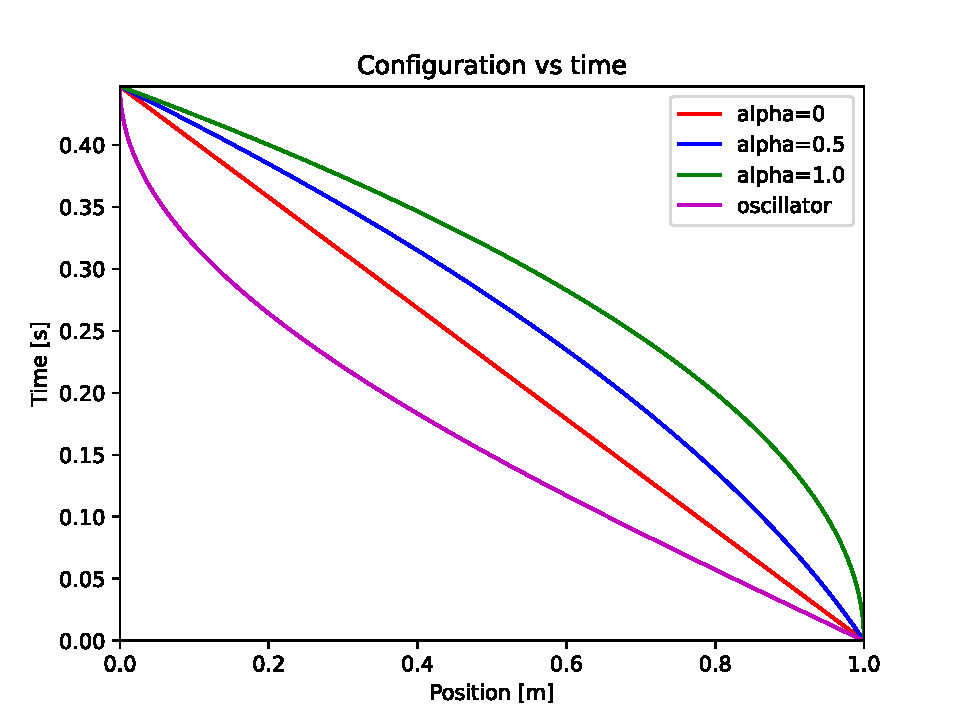
\includegraphics[scale=0.7]{lagrange_vertical}
	\caption{Different types of vertical motion in Lagrange
		picture. Particles start and stop at the same times and in the
		same places, moving between initial and final configurations
		according to different equation $q(t)$.}
	\label{fig:lagrange_vertical}
\end{figure}


It is not difficult to see that the velocity for this general motion
is given by similar combination of velocities:
\[
v_\alpha(t) = \alpha v_a + (1-\alpha)v_c\,.
\]

Let's calculate the Lagrange function for a body moving freely,
without any forces acting on it. Then the Lagrange function is simply
its kinetic energy:
\[
L(t) = \frac{mv_\alpha^2}{2} = \frac{m}{2}\left\lbrack\alpha^2v_a^2+(1-\alpha)^2v_c^2+2\alpha(1-\alpha)v_av_c\right\rbrack\,.
\]
Plugging in the expressions for velocity, we arrive at
\[
L(t) = \frac{m}{2}\left\lbrack\alpha^2a^2t^2+(1-\alpha)^2u^2+2\alpha(1-\alpha)aut\right\rbrack\,.
\]
Now we can calculate the total action accumulated during the motion
from $t=0$ to $t=T$:
\[
A = \int L(t)\delta t = \alpha^2S_1 + (1-\alpha)^2S_2+\alpha(1-\alpha)S_3\,.
\]
Here we denoted
\[
S_1 = \frac{ma^2}{2}\int t^2\delta t\,,\qquad  S_2 = mu^2\int \delta t
\,,\qquad S_3= 2mau \int t\delta t\,.
\]
Examining the expression for the total action, we see that $A$ depends
on the ``mixing'' parameter $\alpha$ in a quadratic way:
\[
A(\alpha) = (S_1+S_2-S_3)\alpha^2 + (S_3-2S_2)\alpha  + S_2\,.
\]
The sums can be evaluated:
\[
S_1 = \frac{ma^2}{2}\frac{T^3}{3}\,,\qquad S_2 =
mu^2T=\frac{mh^2}{T}\,,\qquad S_3 = mauT^2 = mahT\,.
\]
Recalling that $T=\sqrt{2h/a}$ and therefore $h=aT^2/2$, we find
\[
S_3 - 2S_2 = (ma^2T^3/2) - 2ma^2T^4/(4T) = 0\,.
\]
The coefficient in front of $\alpha^2$ is
\[
S_1 + S_2 - S_3 = \frac{ma^2T^3}{6} + \frac{ma^2T^3}{4} -
\frac{ma^2T^3}{2} = -\frac{ma^2T^3}{12}\,.
\]
Finally, the total action depends in the parameter $\alpha$ as
\[
A = \frac{ma^2T^3}{12}(3-\alpha^2)\,.
\]
To find the condition for extremal/stationary action, we need to find
$\alpha$ that maximizes or minimizes the action. Since $A(\alpha)$ is
the inverted parabola with maximum at $\alpha=0$, the maximal action
is achieved for the motion $q_0(t)$ with constant speed without
acceleration and forces.
\begin{exercise}
	Consider the Lagrange function for a body moving under the force of
	gravity:
	\[
	L = \frac{mv^2}{2} - mgq\,.
	\]
	Calculate $L(t)$ for $q_\alpha(t)$ and then calculate total action
	accumulated between $t=0$ and $t=T$. Find $\alpha$ for which the
	action $A(\alpha)$ becomes stationary.
\end{exercise}

\begin{figure}[htbp]
	\centering
	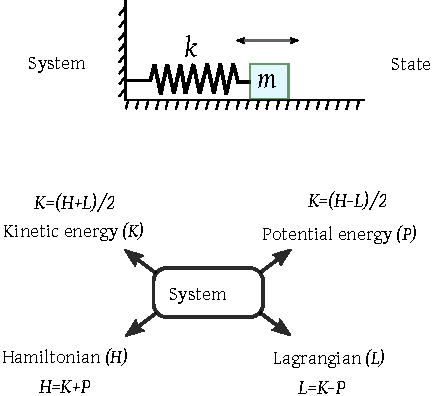
\includegraphics[scale=1.0]{systemDescriptions}
	\caption{System can be described either by kinetic and potential
		energies, or Hamiltonian, or Lagrangian.}
	\label{fig:systemDescriptions}
\end{figure}
\begin{exercise}
	Consider the following ways of traveling from the height $y=h$ to the ground $y=0$ in time $T$:
	\[
	q_1(t) = h - gt^2/2\,,
	\]
	\[
	q_2(t) = h(1 - t/T)\,,
	\]
	\[
	q_3(t) = h\left(1-\sin\frac{\pi t}{2T}\right)\,,
	\]
	\[
	q_4(t) = h\frac{ee^{-t/T}-1}{e-1}\,,
	\]
	and
	\[
	q_5(t) = h(1 - t/T)^2\,.
	\]
\end{exercise}
\subsection{Summary of Three Mechanics}
Let's review what we've learned about three different approaches to study dynamics.
\begin{figure}[htbp]
	\centering
	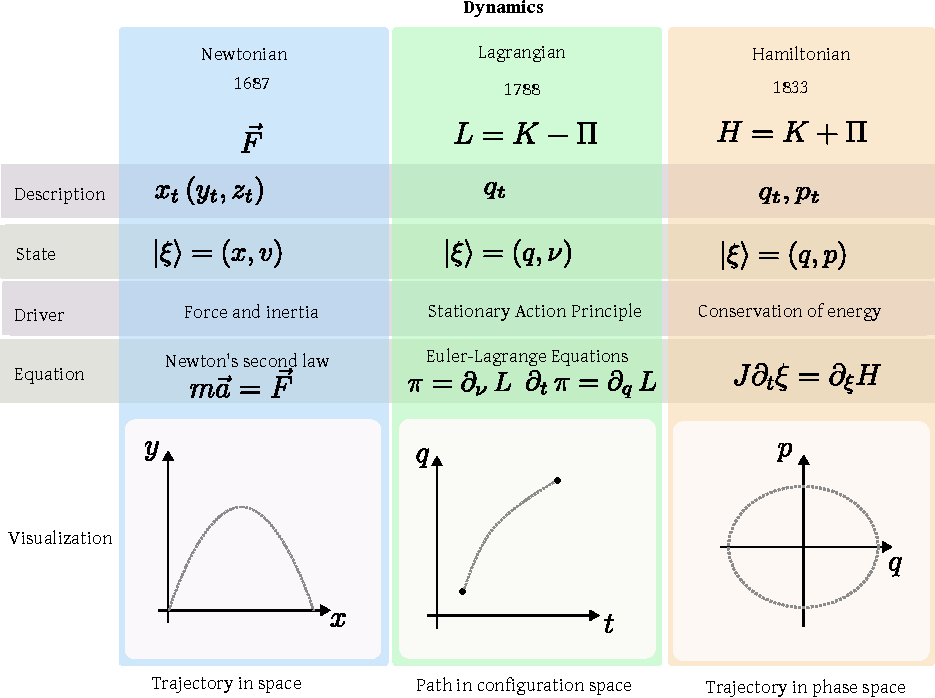
\includegraphics[scale=0.7]{threeMechanics}
	\caption{Summary of three different approaches to problems of motion.}
	\label{fig:threeMechanics}
\end{figure}

State is $\ket{\xi}=(q, u)$ where $q$ is the generalized coordinate and $u=\partial_t\, q$ is \emph{generalized velocity}.
Generalized momentum:
\[
\pi = \partial_u\,L\,,
\]
Euler-Lagrange equation:
\[
\partial_t\,\pi = \partial_q\,L\,.
\]

\section{Field}\label{sec:Field}
In physics, \emph{field} is a \emph{dynamical system} with infinite number of degrees of freedom. It's dynamics can be studied using either Lagrangian or Hamiltonian approach.

\section{Ideal Versus Real}\label{sec:IdealVsReal}
An action of an operator $F$ on arrows can be represented symbolically
as an equation.



\section*{Chapter Highlights}
{\setstretch{1.5}\chhc
  \it  
\begin{itemize}
\item Operators extends the idea of functions.
\item Numeric functions (e.g., $\sin\,x$) act on numbers and yield
  other numbers. Operators may act on vectors to yield other vectors
  or numbers.
\item Linear operators represent the simplest and yet powerful class
  of operators on vectors.
\item Linear operators can be represented graphically or symbolically.
\end{itemize}

}
